\documentclass{ctexart}
\usepackage{graphicx}
\graphicspath{{fig/}}
% \usepackage{caption}
% \usepackage{subcaption}

% 标题控制(caption,bicaption等宏包)
% 并排与子图表(subcaption,subfigure,floatrow等宏包)
% 绕排(picinpar,wrapfig等宏包)

% \begin{tabular}[<垂直对齐方式>]{<列格式说明>}
    % <表项> & <表项> & <表项> & ... & <表项> \\
    % ...... 
% \end{tabular}
% 用\\表示换行
% 用&表示不同列
% l-列左对齐
% c-列居中对齐
% r-列右对齐
% p{<宽>}-列宽度固定,超过宽度的自动换行

% 浮动体
% 实现灵活分页(避免无法分割的内容产生的页面留白)
% 给图表添加标题
% 交叉引用

% figure环境(table环境与之类似)
% \begin{figure}[<允许位置>]
%     <任意内容>
% \end{figure}

% <允许位置>参数(默认tbp)
% h,此处(here)-代码所在的上下文位置
% t,页顶(top)-代码所在的页面或之后页面的顶部
% b,底部(buttom)-代码所在的页面或之后页面的底部
% p,独立一页(page)-浮动页面

\begin{document}
    成绩表见表\ref{table1}。

    \LaTeX{}的插图1:
    \begin{figure}[htbp]
        \centering
        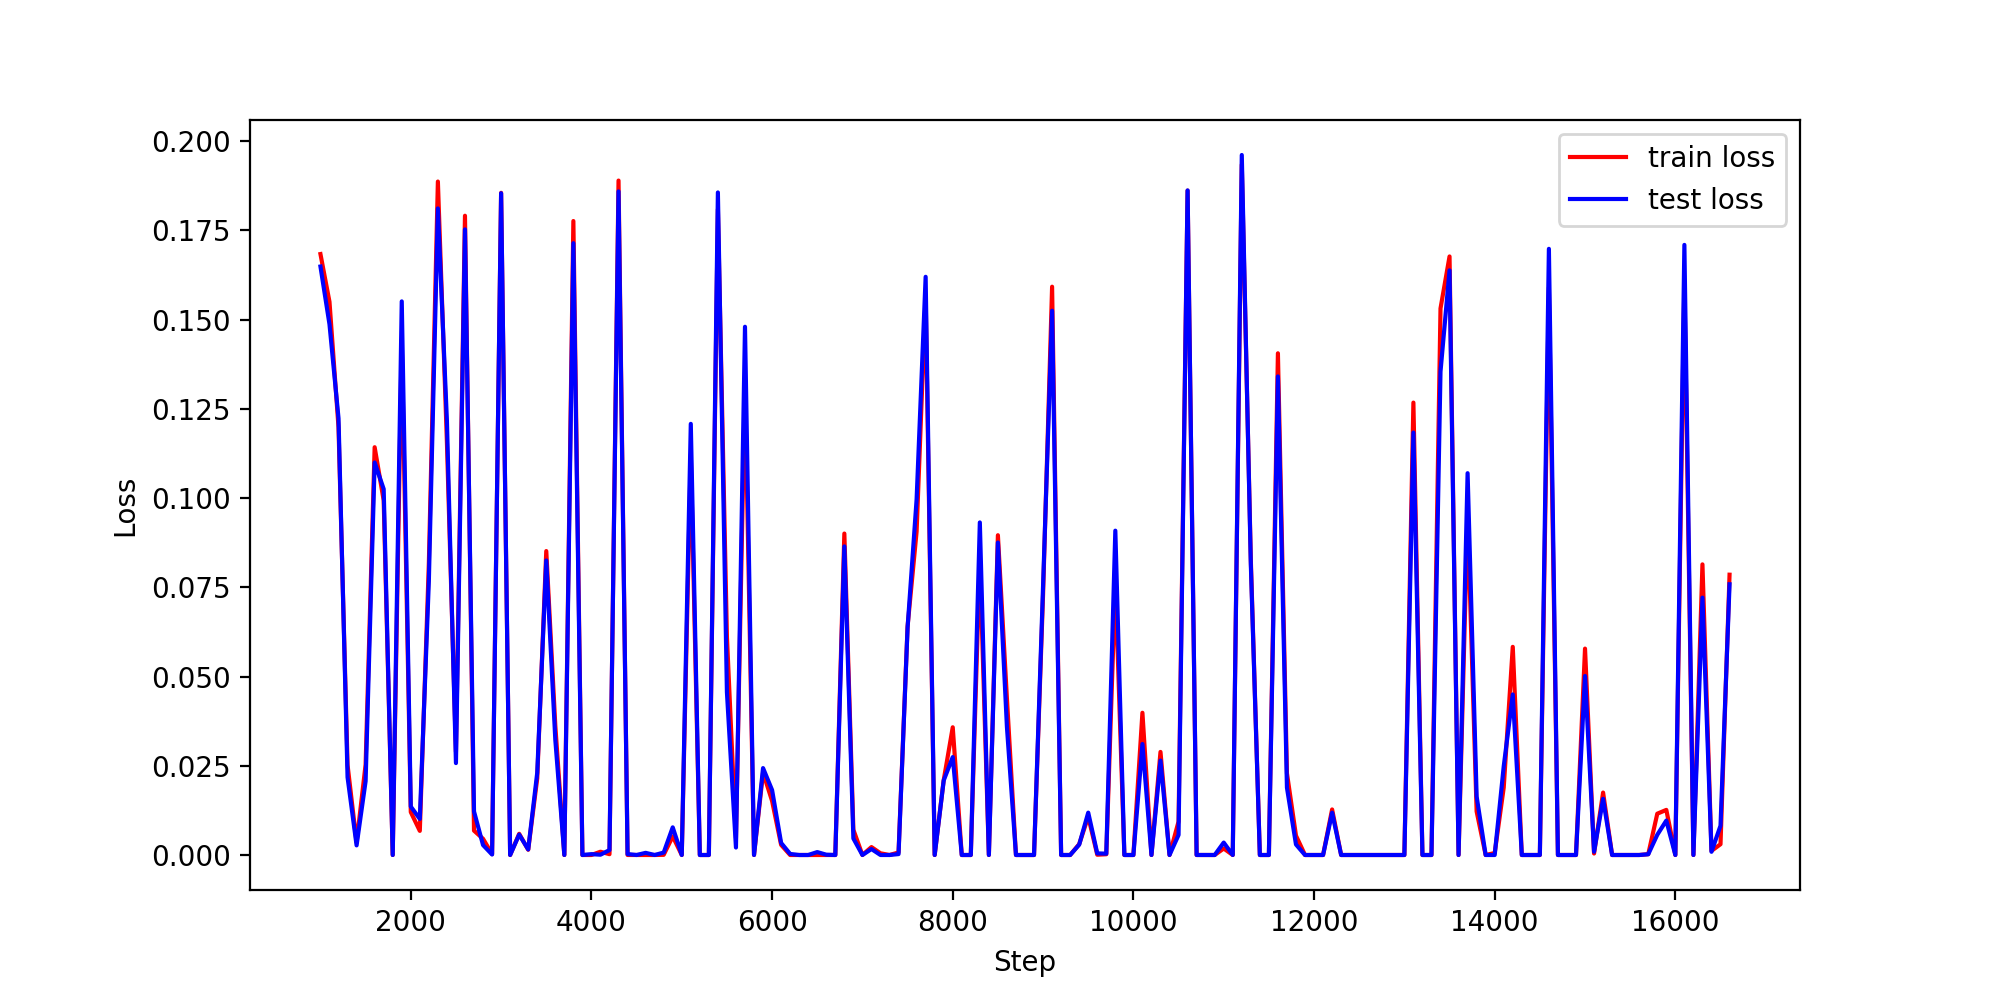
\includegraphics[scale=0.3]{st_250}
        \caption{loss of st\_250}
    \end{figure}
    

    \LaTeX{}的表格1:
    \begin{table}[h]
        \centering
        \caption{成绩表}\label{table1}
        \begin{tabular}{|l|c|c|c|r|}
            \hline
            姓名 & 语文 & 数学 & 外语 & 备注 \\
            \hline
            张三 & 87 & 100 & 64 & 优秀 \\
            \hline
            李四 & 75 & 88 & 52 & 补考另行通知 \\
            \hline
            王五 & 60 & 90 & 80 & \\
            \hline
        \end{tabular}
    \end{table}
    
    \begin{figure}[h]
        \centering
        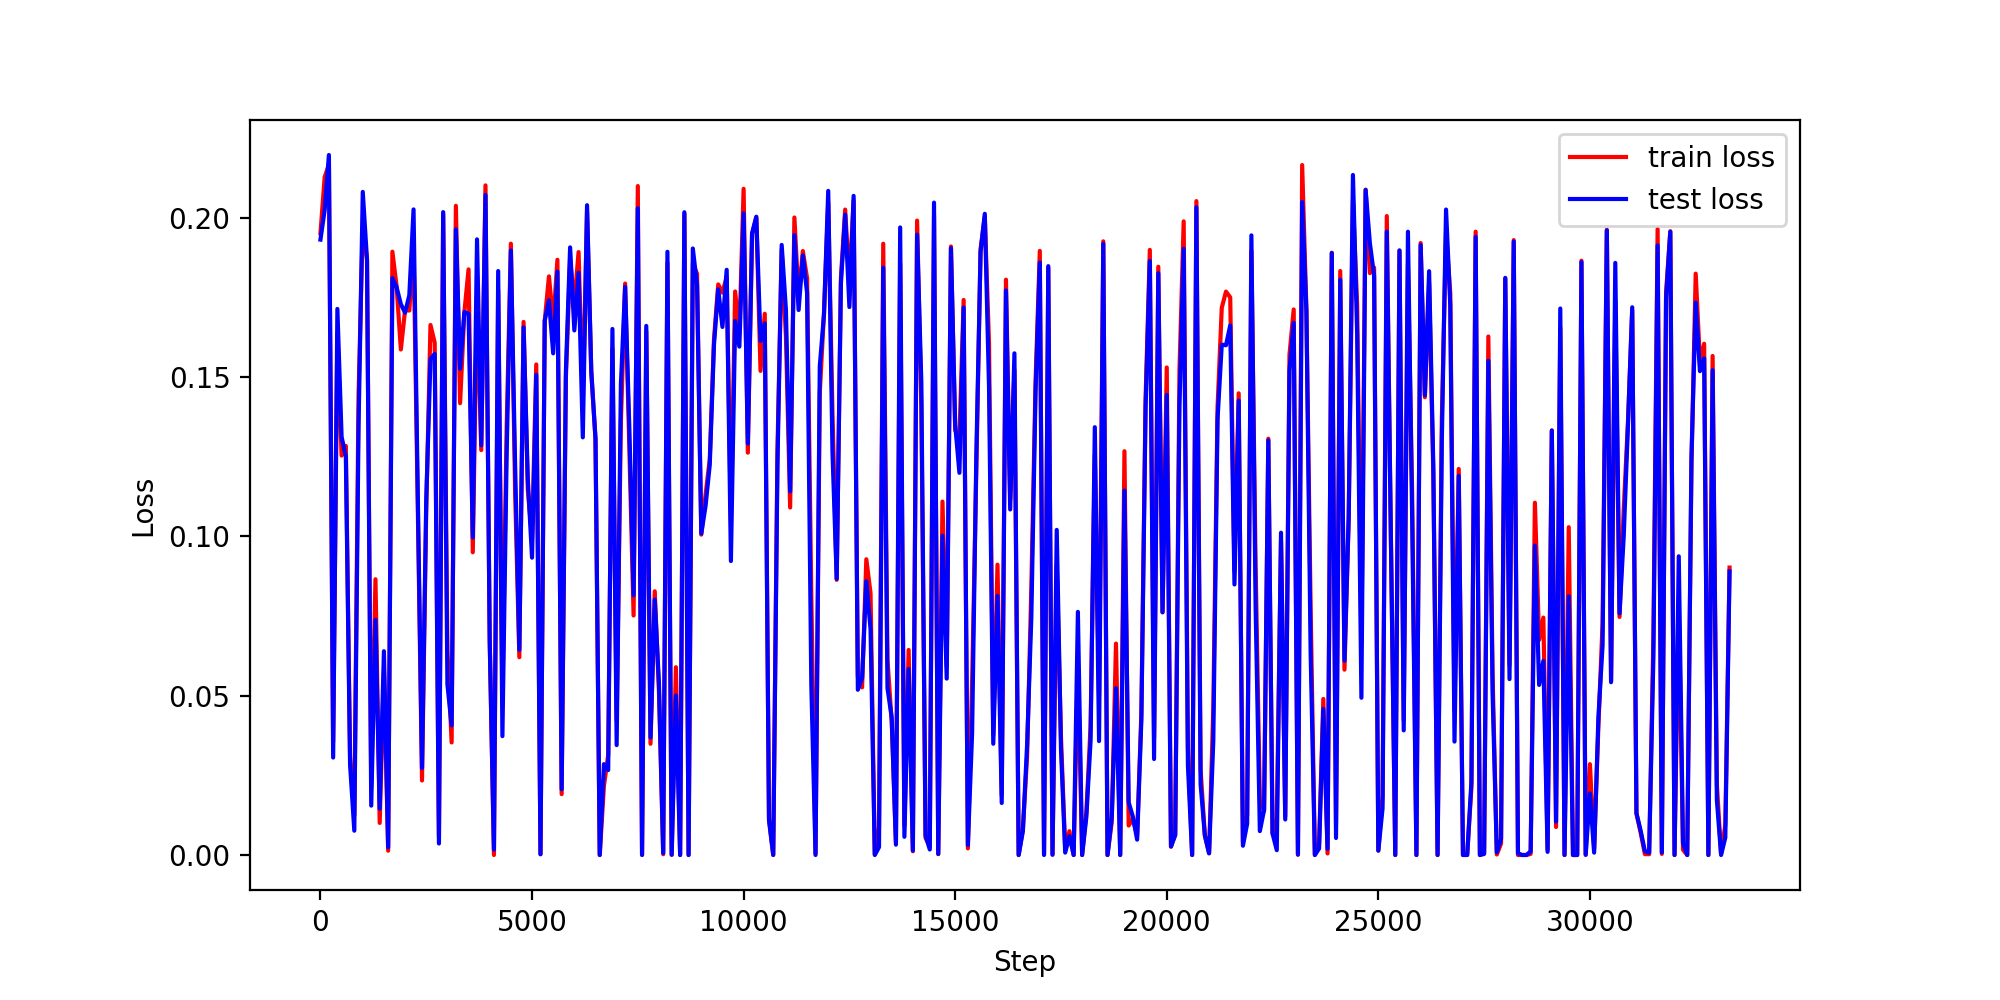
\includegraphics[scale=0.3]{thchs(1).png}
        \caption{loss of thchs(1)}
    \end{figure}

    \begin{figure}[h]
        \centering
        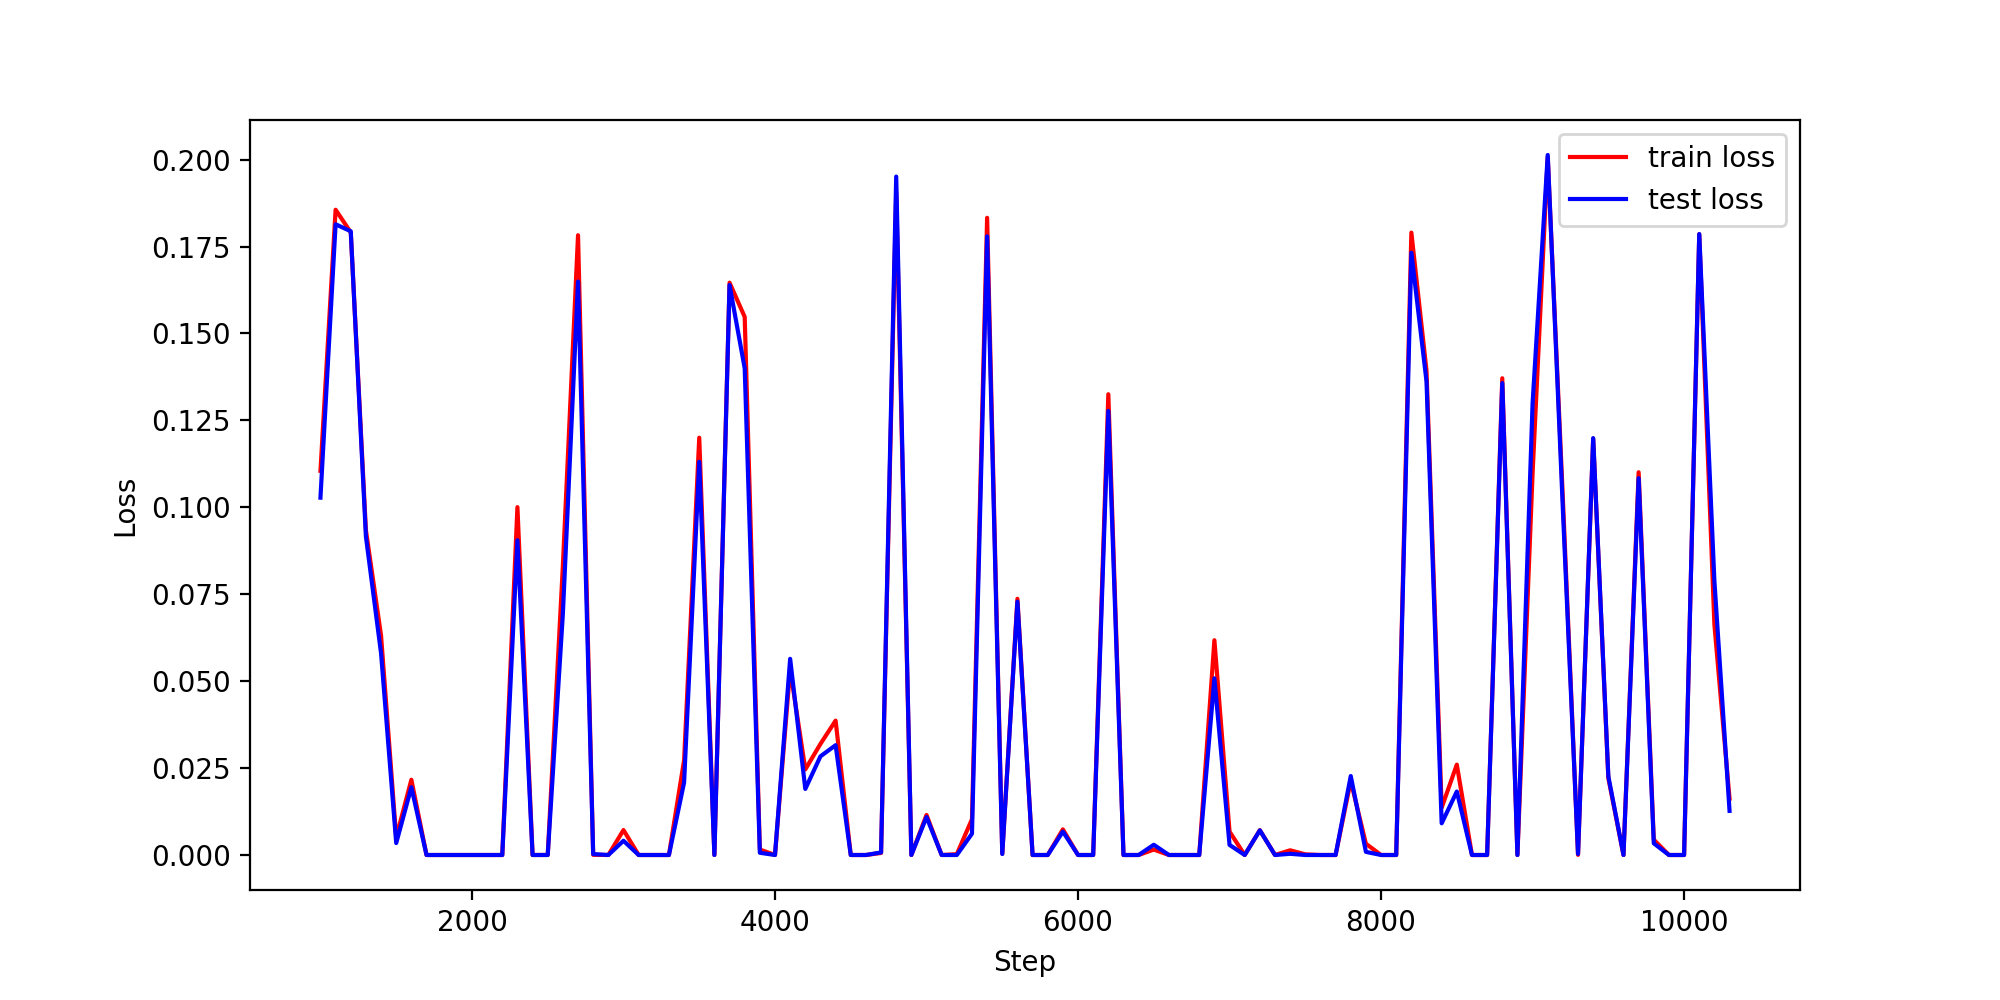
\includegraphics[scale=0.3]{thchs(2).png}
        \caption{loss of thchs(2)}
    \end{figure}

    \begin{figure}[h]
        \centering
        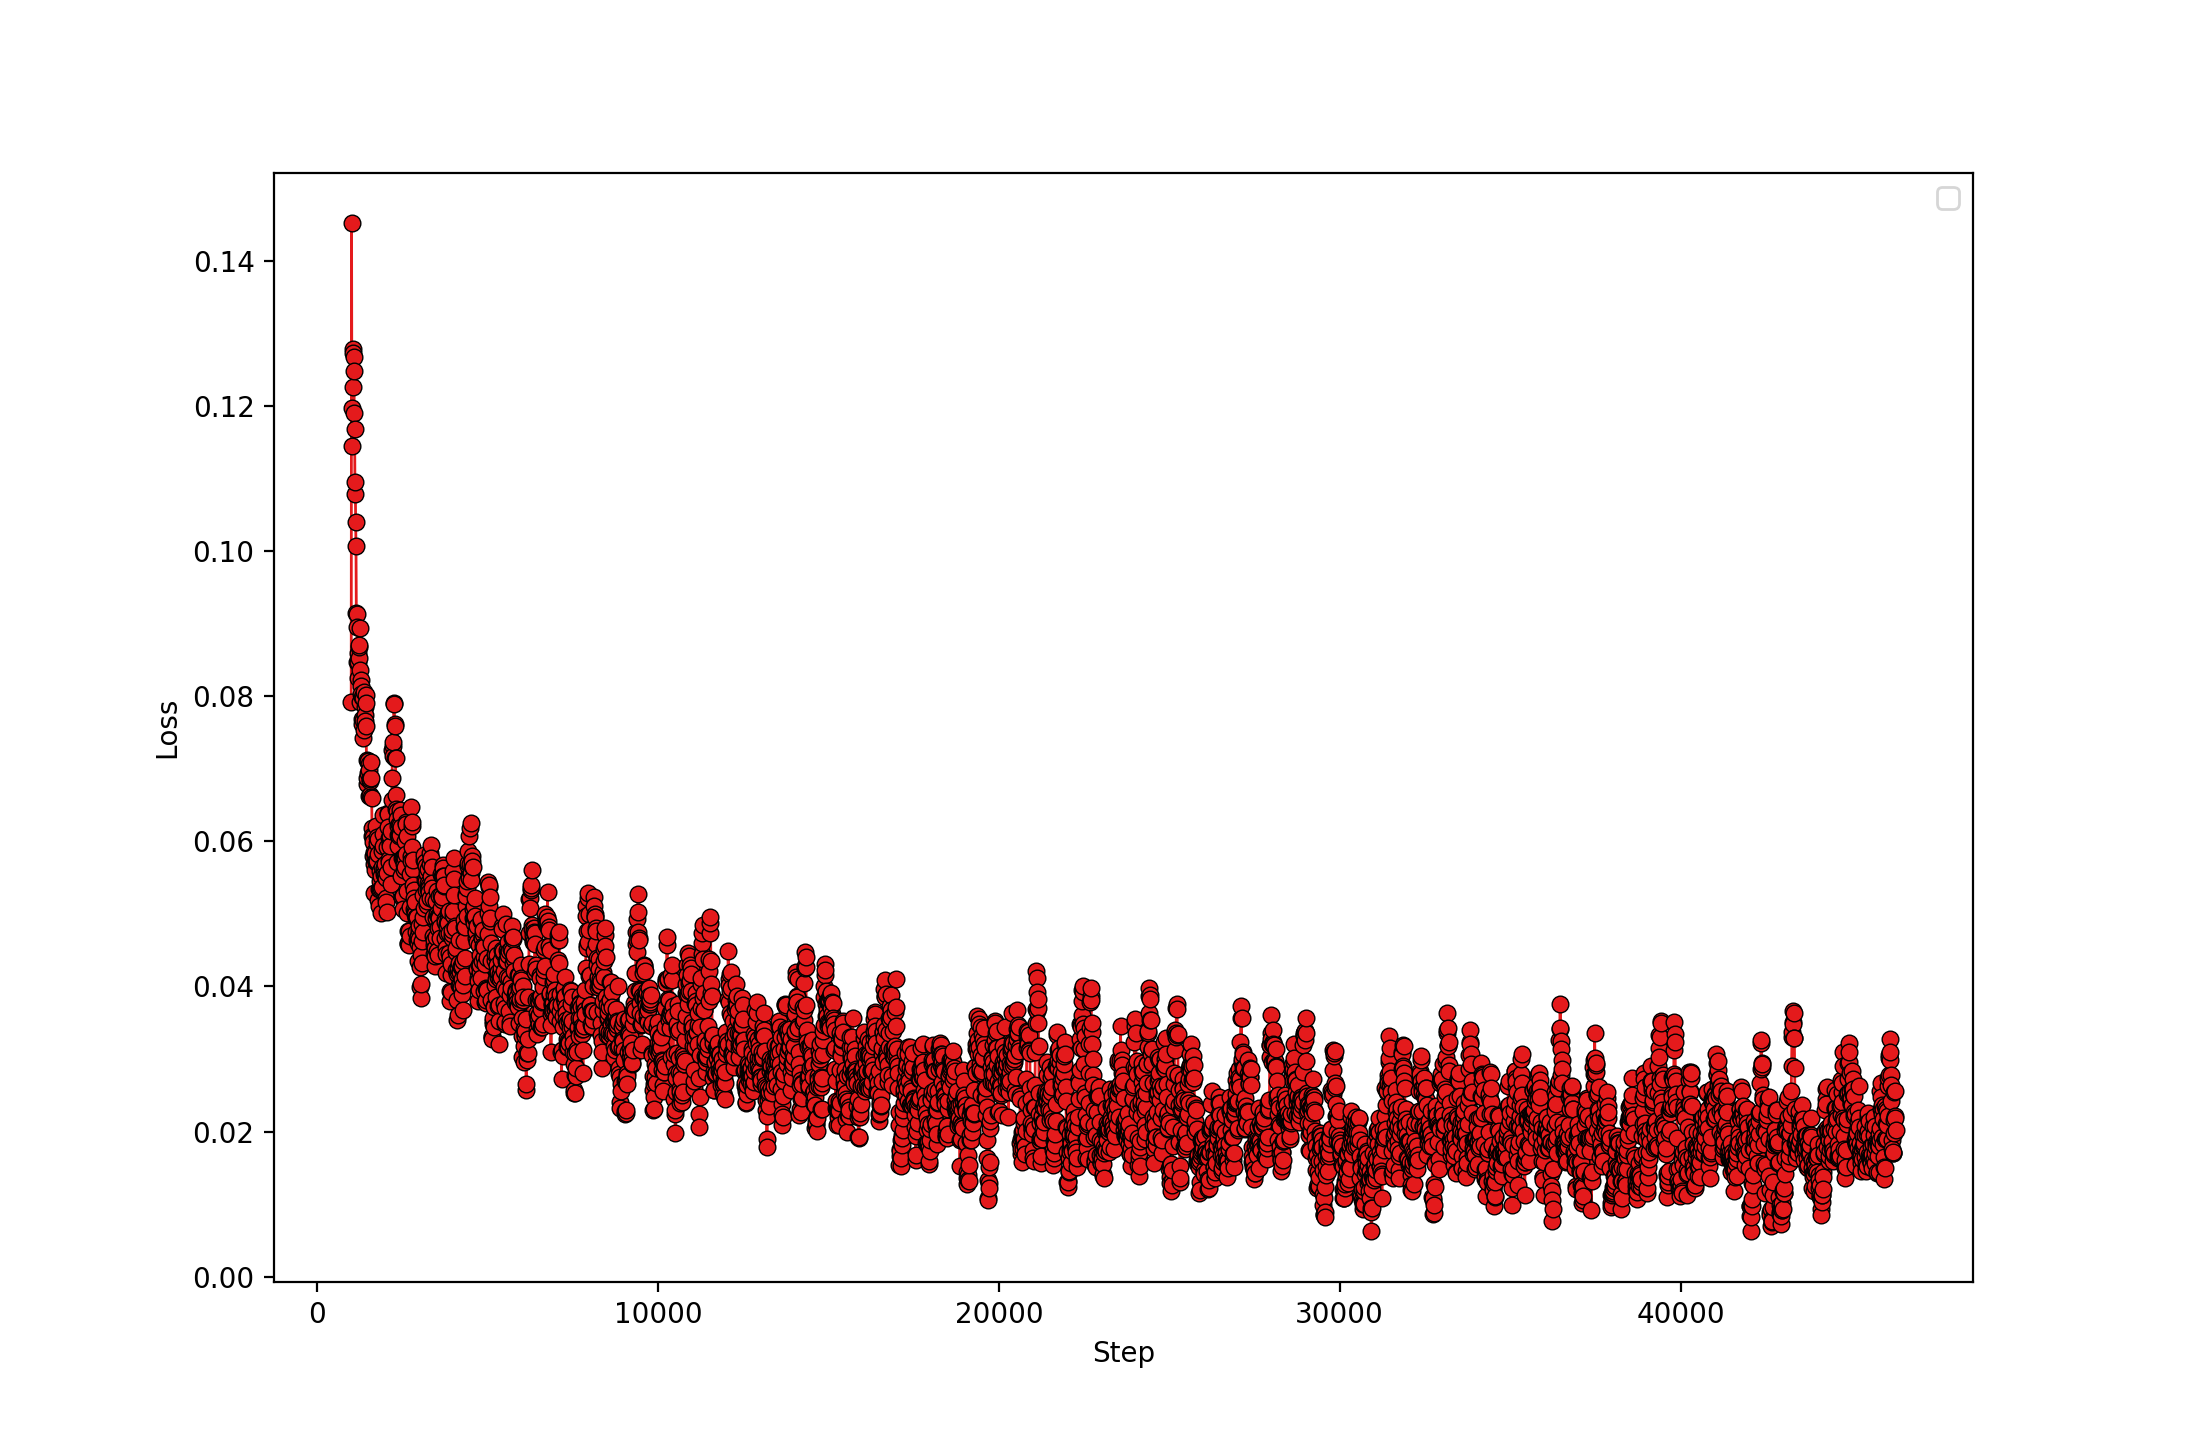
\includegraphics[scale=0.3]{vctk.png}
        \caption{loss of vctk}
    \end{figure}

    \begin{figure}[h]
        \centering
        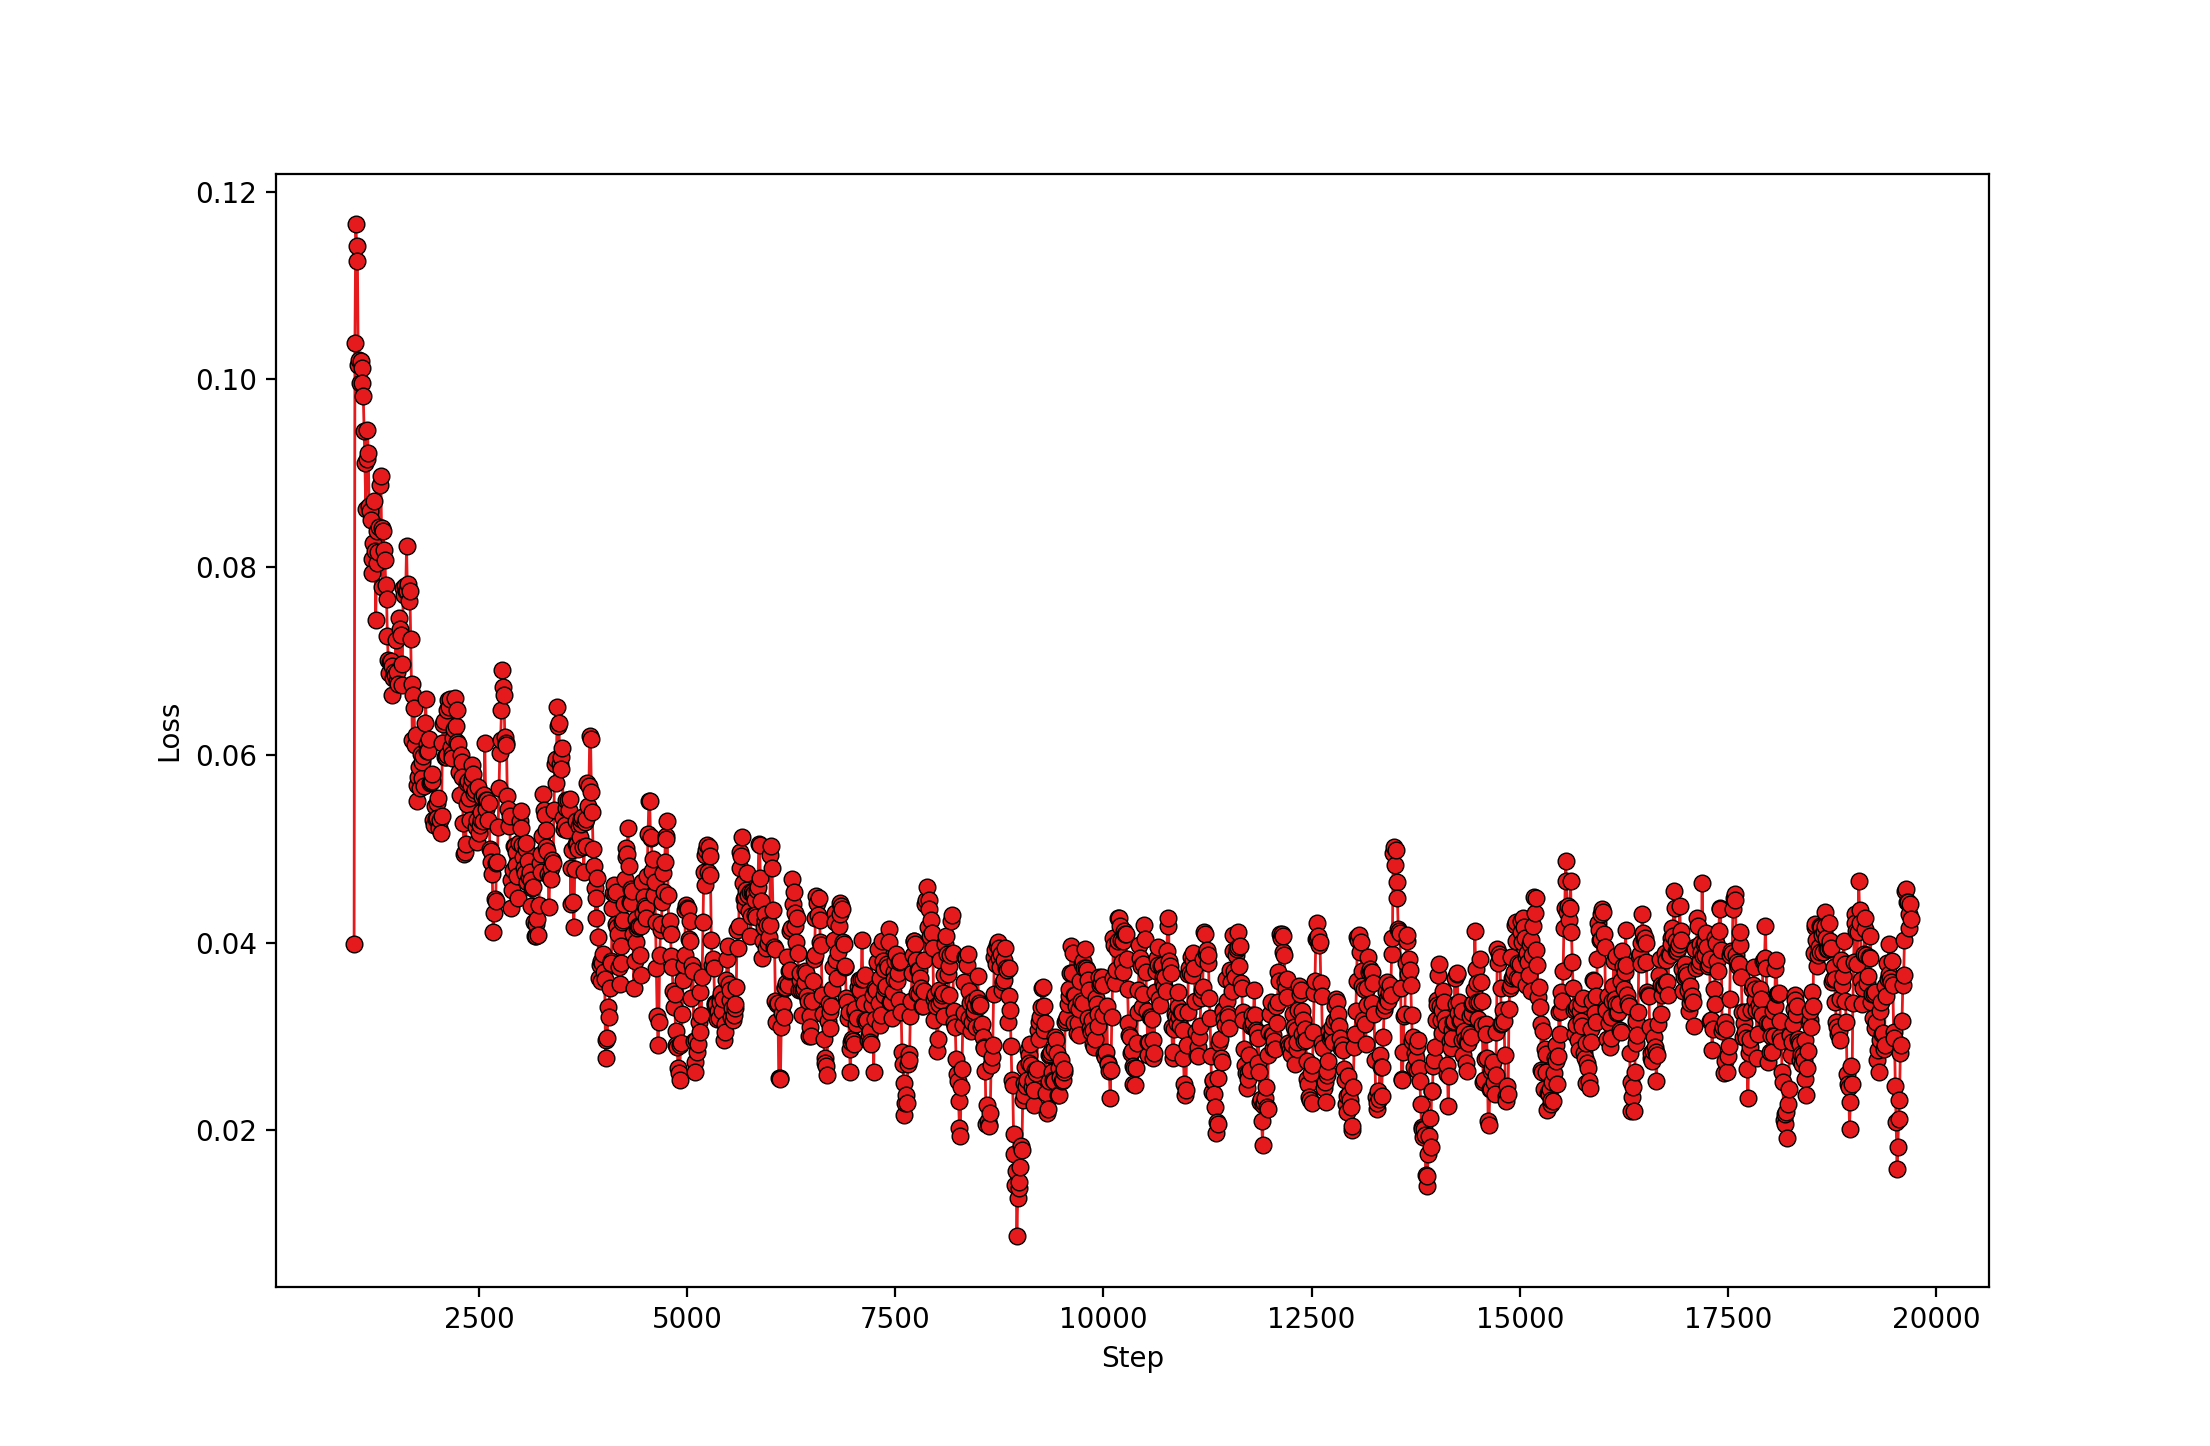
\includegraphics[scale=0.3]{thchs(3).png}
        \caption{loss of thchs(3)}
    \end{figure}

\end{document}